\documentclass[a4paper, 9pt]{scrartcl}
\usepackage{geometry}                % See geometry.pdf to learn the layout options. There are lots.                  % ... or a4paper or a5paper or ... 
%\geometry{landscape}                % Activate for for rotated page geometry
\usepackage[parfill]{parskip}    % Activate to begin paragraphs with an empty line rather than an indent
\geometry{verbose,tmargin=0.6in,bmargin=0.7in,lmargin=0.8in,rmargin=0.8in}
\usepackage{graphicx}
\usepackage{amssymb}
\usepackage{amsthm}
\usepackage{epstopdf}
\usepackage{mathtools}
\usepackage[shortlabels]{enumitem}
\usepackage{dsfont}
\usepackage{sidecap}
\usepackage[usenames,dvipsnames]{color}
\usepackage[thinspace,mediumqspace,Grey,squaren]{SIunits}
\usepackage{bbm}
\DeclareGraphicsRule{.tif}{png}{.png}{`convert #1 `dirname #1`/`basename #1 .tif`.png}




%\def\thesection{D.\arabic{section}}
%\def\thefigure{D.\arabic{figure}}
%\def\thetable{D.\arabic{table}}

\begin{document}



%%%% Commands

\newcommand{\vect}[1]{\mathbf{#1}}
\newcommand{\vectSymbol}[1]{\boldsymbol{#1}}

\newcommand{\Normal}[2]{\mathcal{N}\left( #1, #2 \right)}


%%%% Definitions

\def\MCChain{\Lambda}
\def\mCChain{\lambda}
\def\mCChainInt{\boldsymbol{\lambda}}
\def\MCIndex{j}


\def\Time{t}
\def\TimeIndex{N}
\def\timeIndex{l}
\def\DiscreteTime{\Time_{\timeIndex}}

\def\InitialDistribution{\pi}
\def\ParameterPrior{\phi}
\def\SingleParamPrior{\phi}
\def\MeasurementParamPrior{\psi}
\def\SingleMeasurementParamPrior{\psi}

\def\MeasurementSigma{\Sigma}
\def\measurementSigma{\sigma}

\def\Joint{p}
\def\Density{p}
\def\Proposal{q}

\def\GammaDistribution{\mathcal{G}}

\def\noise{u}
\def\Noise{U}


\def\NExtrinsic{N}
\def\extrinsicVariable{z}
\def\ExtrinsicVariable{Z}
\def\ExtrinsicSpace{\mathcal{Z}}
\def\hyperParameters{a}
\def\HyperParameters{A}
\def\HyperSpace{\mathcal{A}}


\def\MarkovChain{\State}
\def\State{X}
\def\StatePopulation{\mathbb{X}}
\def\StateInt{\mathbf{\State}}
\def\state{x}
\def\stateInt{\mathbf{\state}}
\def\StateTime{\State({\Time})}
\def\stateDiscreteTime{\state_{\timeIndex}}
\def\StateDim{d}
\def\ReactionDim{\nu}
\def\CellCount{M}
\def\StateSpace{\mathbb{N}_{+}}
\def\StateSpaceDim{\StateSpace^{\StateDim}}

\def\Measurement{Y}
\def\MeasurementInt{{\Measurement}}
\def\measurement{y}
\def\measurementInt{{\measurement}}
\def\MeasurementTime{\Measurement_{\timeIndex}}
\def\measurementTime{\measurement_{\timeIndex}}
\def\MeasurementDim{o}
\def\MeasurementSpace{\mathbb{R}}
\def\MeasurementSpaceDim{\MeasurementSpace^{\MeasurementDim}}

\def\PathDensity{f}
\def\MeasurementDensity{g}

\def\AllParameters{\Theta}
\def\allParameters{\theta}

\def\SharedParameters{S}
\def\sharedParameters{s}

\def\kParameters{C}
\def\kparameters{c}
\def\kparameter{c}

\def\Lapvar{\sigma}

% marginal propensity
\def\MargProp{h}

\def\Parameters{C}
\def\parameters{c}
\def\parameter{c}

\def\MeasurementParameters{\Omega}
\def\measurementParameters{\omega}

\def\Covariates{V}
\def\covariates{v}

\def\GammaDist{\mathcal{G}}

% the differential sign should not be italic
\def\df{\mathrm{d}}

\def\MarkovBlanket{\mathcal{MB}}

\def\History{\mathcal{H}}

%% Spaces
\def\Real{\mathbb{R}}
\def\RealPos{\mathbb{R}_{\geq 0}}

\def\FullLatentSet{U}
\def\fullLatentSet{u}
\def\FullMeasurementSet{Z}
\def\fullMeasurementSet{z}
\def\LatentSubSet{\FullLatentSet}
\def\latentSubSet{\fullLatentSet}

\newcommand{\Expect}[1]{ \mathbb{ E } \left[ #1 \right]}
\newcommand{\ExpectWRT}[2]{ \mathbb{ E }_{ #2 } \left[ #1 \right]}
\newcommand{\Var}[1]{ \mathrm{Var} \left[ #1 \right]}
\newcommand{\VarWRT}[2]{ \mathrm{ Var }_{ #2 } \left[ #1 \right]}

\def\Mgf{G}

\def\PriorParameters{\Theta}
\def\priorParameters{\theta}
\def\priorParamA{\kappa}
\def\priorParamB{\chi}
\def\PathSpace{\mathcal{X}}

\newcommand{\LogNormal}[2]{\mathcal{LN} \left( #1, #2 \right)}
\newcommand{\Uniform}[2]{\mathcal{U} \left( #1, #2 \right)}

\def\Model{\mathcal{M}}
\def\model{m}
\def\BayesFactor{\mathcal{K}}

\def\IndexSet{\mathcal{I}}
\def\CylinderSet{\Gamma(\stateInt)}

\def\MorphParameters{B}
\def\morphParameters{b}

\newcommand{\Indicator}[2]{\mathbbm{1}_{#2} \left( #1 \right)}


\newcommand{\Comment}[2]{ {\color{blue} #1} \textit{Remark: #2}}



\def\DPP{DPP~}
\def\GuiDPP{GuiDPP~}

\title{A Tutorial on \DPP and \GuiDPP}
\date{}
\maketitle



\tableofcontents

\newpage

\section{Requirements and Installation}

\begin{itemize}
	\item Working MATLAB installation (toolbox tested with MATLAB2012b).
	\item 64bit MacOS, Windows or Linux.
	\item Extract the zip-archive that you have downloaded to a desired location \textit{PATH}. 
\end{itemize}

\section{\GuiDPP}

\GuiDPP is a MATLAB application based on the \DPP toolbox with a graphical user interface (GUI). While \DPP applies to arbitrary biochemical systems, \GuiDPP was specifically designed for calibrating heterogeneous gene expression systems that are regulated by a transient stimulus (e.g., such as the translocation of a transcription factor).

\subsection{Starting \GuiDPP}

Start MATLAB and open the script \textit{PATH/GUI/StartGUI.m}. Upon execution of the script, \GuiDPP  pops up and is ready to use. A quick guide with the most important properties and features can be found in Figure \ref{fig:QuickGuide}.

\begin{figure}[htbp]
\begin{center}
	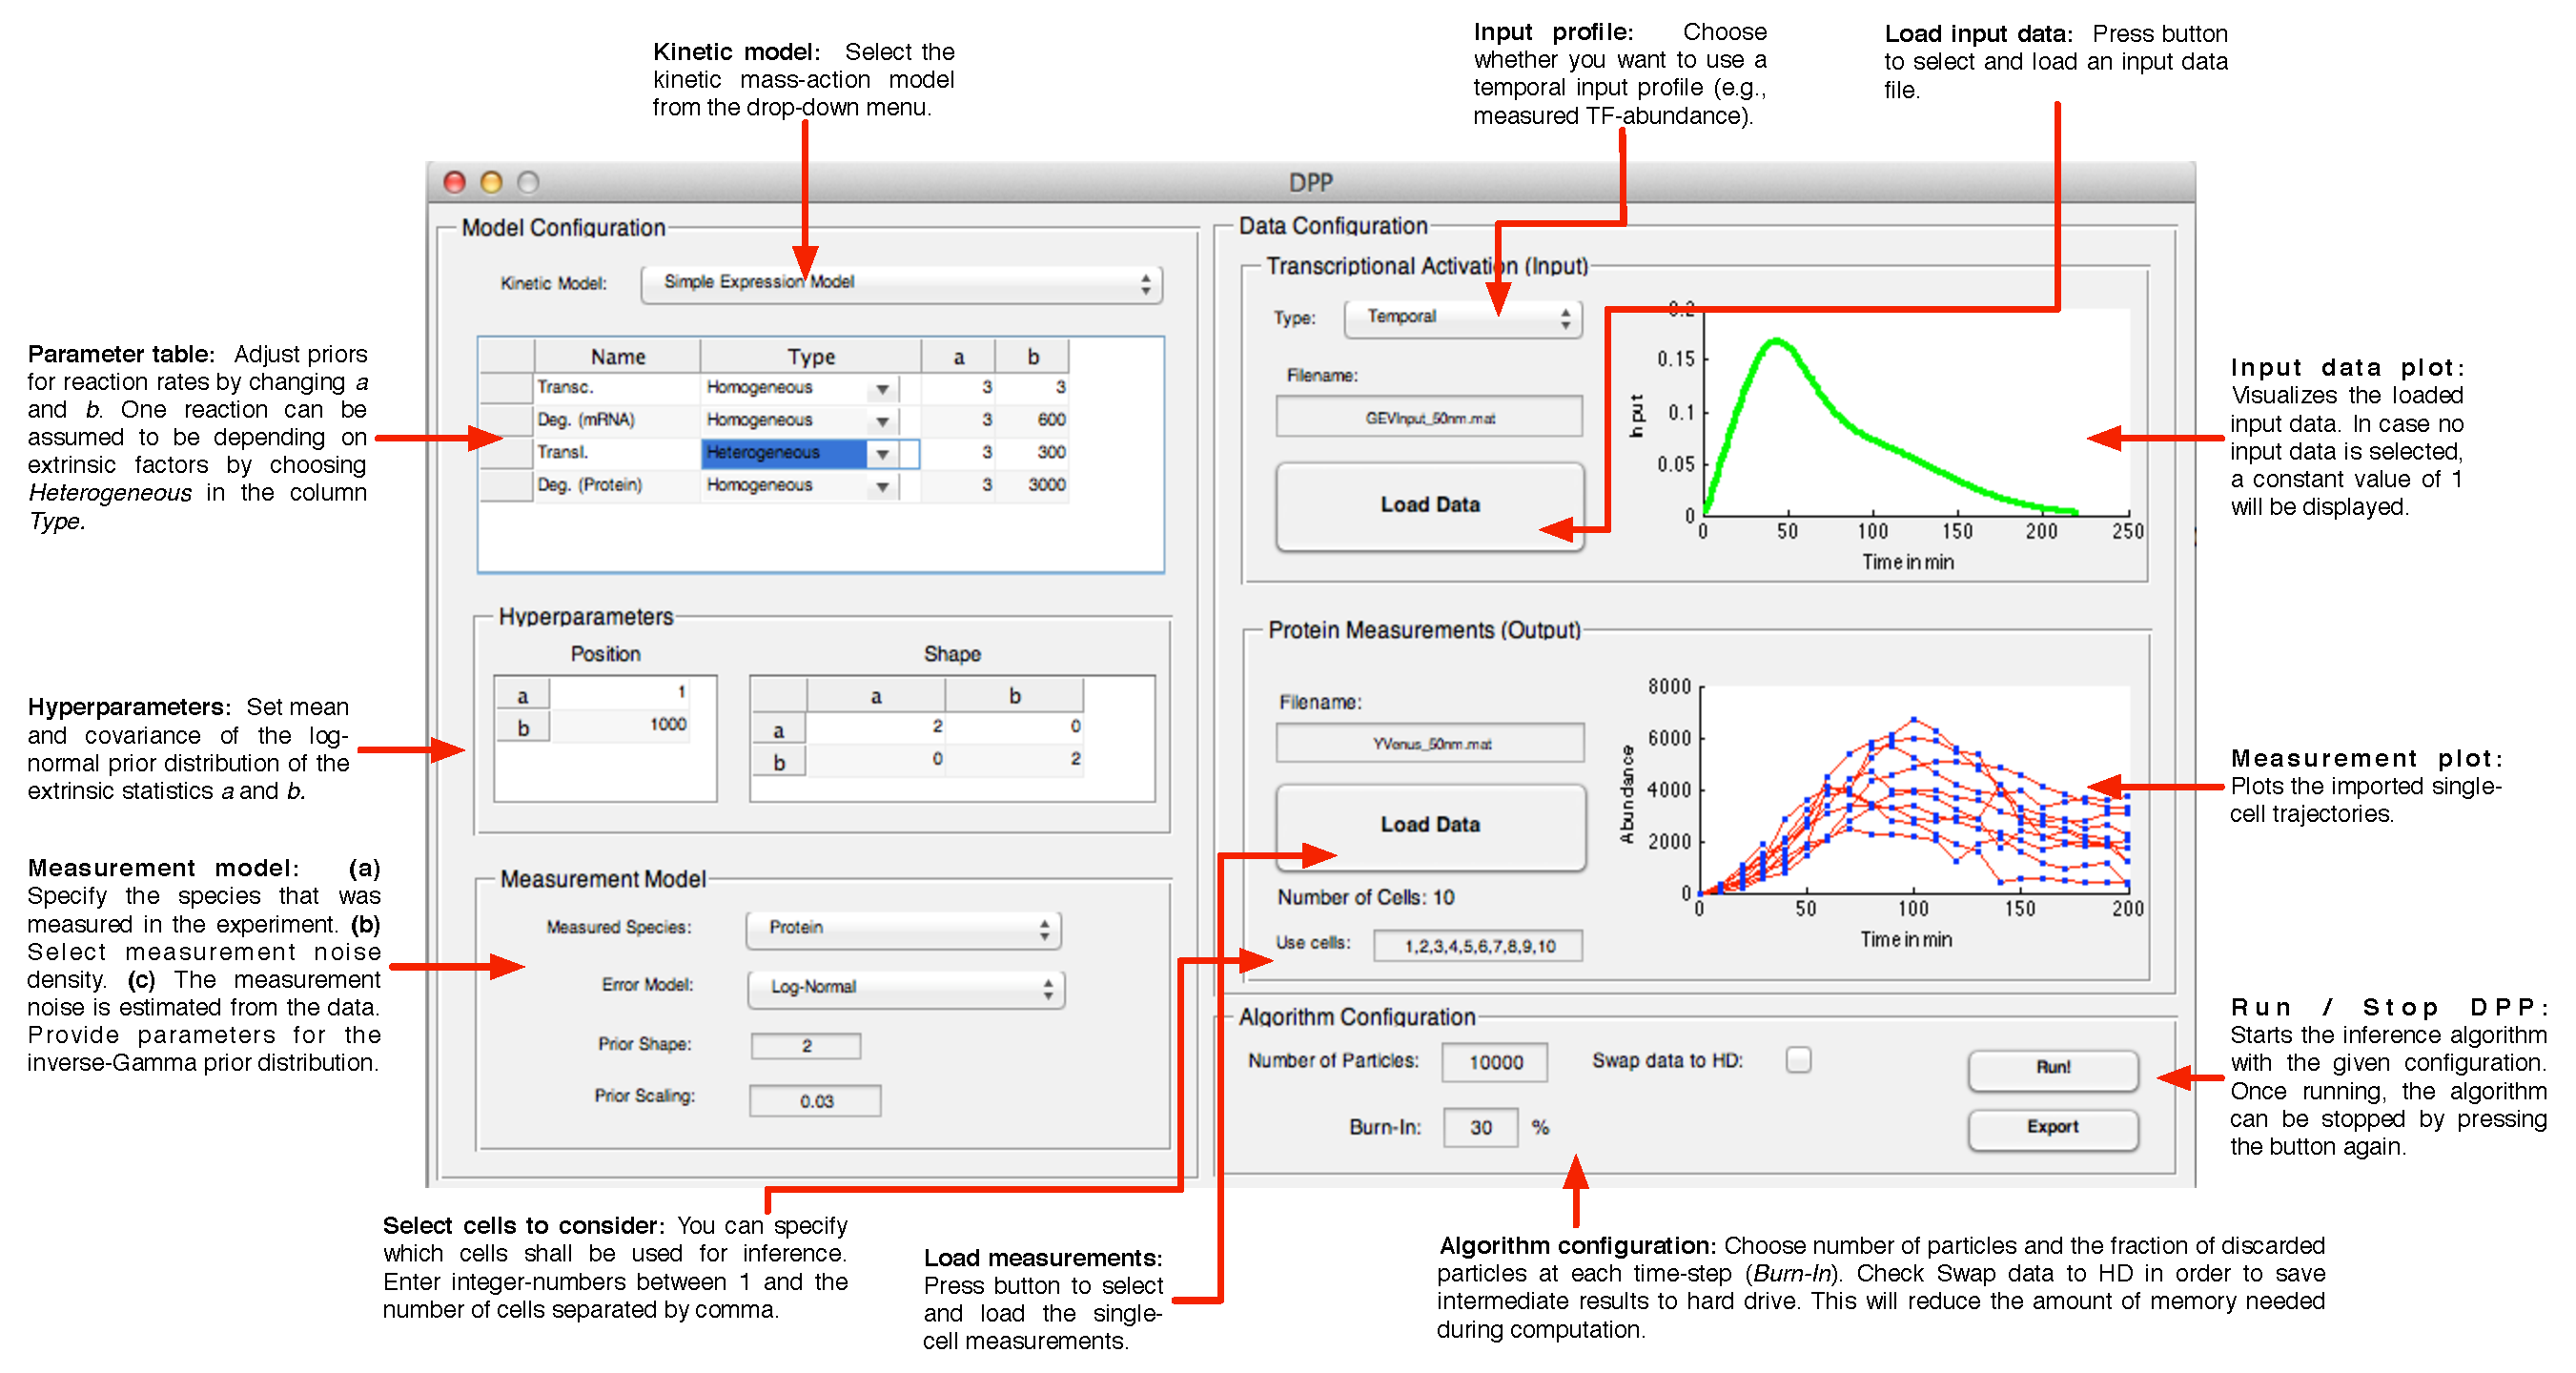
\includegraphics[width=0.999\textwidth]{figures/Doc_QuickstartGUI}
\caption{Quick guide for \GuiDPP.}
\label{fig:QuickGuide}
\end{center}
\end{figure}

\subsection{How to use \GuiDPP}
\label{sec:HowToGuiDPP}

\paragraph{Kinetic model and parameters:} \GuiDPP automatically loads all models from \textit{PATH/Models/} and displays them in the corresponding drop-down menu. Per default, two gene expression models are available:
\begin{enumerate}
	\item \textbf{Simple Expression Model:} A simple model of transcription and translation given by the reactions:
		\begin{equation}
			\begin{split}
			\emptyset &\xrightleftharpoons[\kparameter_{2}]{\kparameter_{1} u(t) } \text{mRNA} \\
	\text{mRNA} &\xrightharpoonup{\kparameter_3} \text{mRNA} + P \\
	P &\xrightharpoonup{\kparameter_4} \emptyset. \nonumber
			\end{split}
		\end{equation}
	\item \textbf{Two-State Model:} Canonical two-state model including gene-activation and deactivation:
	 	\begin{equation}
			\begin{split}
			G^{off} &\xrightleftharpoons[\kparameter_{2}]{\kparameter_{1} u(t) } G^{on} \\
			G^{on} &\xrightharpoonup{\kparameter_3} G^{on} +  \text{mRNA} \\
			mRNA &\xrightharpoonup{\kparameter_4} \emptyset \\
	\text{mRNA} &\xrightharpoonup{\kparameter_5} \text{mRNA} + P \\
	P &\xrightharpoonup{\kparameter_6} \emptyset. \nonumber
			\end{split}
		\end{equation}
\end{enumerate}
Additional models can be included into \GuiDPP by copying the corresponding \textit{*.mat} files to the \textit{PATH/Models/} folder. The definition of custom models is described in Section \ref{sec:Models}. \newline

Once a model has been selected, the parameter table will be automatically updated. Each row corresponds to a particular kinetic parameter (i.e., stochastic rate constant) and its properties. In the column \textit{Type}, you can select a reaction that is assumed to be driven by extrinsic factors. In this case, choose \textit{Heterogeneous}\footnote{Note that in the current version, only one heterogeneous reaction is supported.}. The columns \textit{a} and \textit{b} are used to specify the Gamma-type prior distributions for the individual parameters. For practical hints on the choice of the prior distributions see Section \ref{sec:Priors}.

\paragraph{Hyperparameters:} If a reaction is chosen to be heterogeneous, the section \textit{Hyperparameters} becomes visible. These parameters will be used to specify the bivariate (hyper)-prior distribution for $(a, b)$ corresponding to the heterogeneous parameter. In particular, a log-normal distribution will be constructed as
\begin{equation}
	p(a, b) \propto \Normal{\ln \mu}{\Sigma}, \nonumber
\end{equation}
with $$\mu = \begin{pmatrix} \mu_{a} \\ \mu_{b} \end{pmatrix}$$ and $$\Sigma = \begin{pmatrix} s_{a} &s_{a, b} \\ s_{a, b} &s_{b}  \end{pmatrix}$$ as the parameter values provided by the user.

\paragraph{Measurement model:} The user can select the chemical species which was measured in the experiment and chose among a normal and log-normal measurement error density. In both cases, the shape parameter of the respective density (e.g., the standard deviation $\sigma$ in case of a normal distribution) is assumed to be unknown and estimated from the data. The prior distribution for the shape parameters is assumed to be inverse-Gamma, which is a conjugate prior for both the normal and the log-normal density. The inverse-Gamma distribution is specified by
\begin{equation}
	I\GammaDistribution(p, q) = \GammaDistribution(p, q^{-1}),
\end{equation}
with $p$ and $q$ as the provided shape and scaling parameters.


\paragraph{Transcriptional Activation (Input):} As described above, the expression of the target gene is assumed to be transiently regulated by a certain \textit{input} stimulus $u(t)$. In case there is no such input (e.g., for constitutively expressed genes), choose \textit{Constant} in the drop-down menu \textit{Type}. If you choose \textit{Temporal}, you can specify and load an external input file. Exemplary input files are provided in the folder \textit{PATH/ExampleData/}. Section \ref{sec:DPP} contains further information on how custom input profiles can be created within MATLAB.

\paragraph{Protein Measurements (Output):} The measurement file can be located and loaded using the \textit{Load Data} button. The individual single-cell traces will be automatically plotted. The text box \textit{Use cells} can be used to select only a subset of the cells. Enter the desired cell-numbers separated by comma. Exemplary measurement files are provided in the folder \textit{PATH/ExampleData/}. Section \ref{sec:DPP} contains further information on how to generate valid measurement files from your custom experimental data.

\paragraph{Algorithm Configuration:} Specify the number of particles used during each time iteration. Note that this value directly influences the execution time and allocated memory. For a quick test run, we recommend to use a small number of particles (e.g., around 500-1000), but keep in mind that the resulting posterior distributions are likely to be degenerate. The parameter \textit{Burn-In} defines the relative amount of particles to be discarded in the underlying Markov Chain Monte Carlo (MCMC) scheme. Typically, a longer burn-in period will be needed if many cells are in place. For large simulations, we recommend to select the \textit{Swap data to HD} options since the data created at runtime can easily reach several gigabytes. In this case, the intermediate posterior distributions at the individual time points will be swapped to your hard drive (i.e., \textit{PATH/GUI/DistTmp\_*}). These files can subsequently be used to reconstruct to full posterior distribution over all time points (see Section \ref{sec:DPP}).%The \textit{Parallel} button can be used to enable parallel execution of the simulations. In particular, it will launch the default MATLAB pool using the \textit{local} configuration.

\paragraph{Starting \DPP:} Once you have finished your configuration you can press \textit{Run!} in order to start the inference algorithm. The caption of the button will now change to \textit{Stop!}, which you can now use to cancel the running simulations. Be aware that both starting and stopping the simulations will require a certain amount of time, depending on your configuration and the number of particles (memory pre-allocation, cleanup, etc.).
After you have started the algorithm, a new window will pop up, which you can use to monitor a running simulation. In particular, it will display the most recent posterior distributions over the states and parameters (see Figure \ref{fig:Monitor}). Note that the posterior distribution over the states will not change (i.e., will be empty) until the first time iteration has completed.
\begin{figure}[htbp]
\begin{center}
	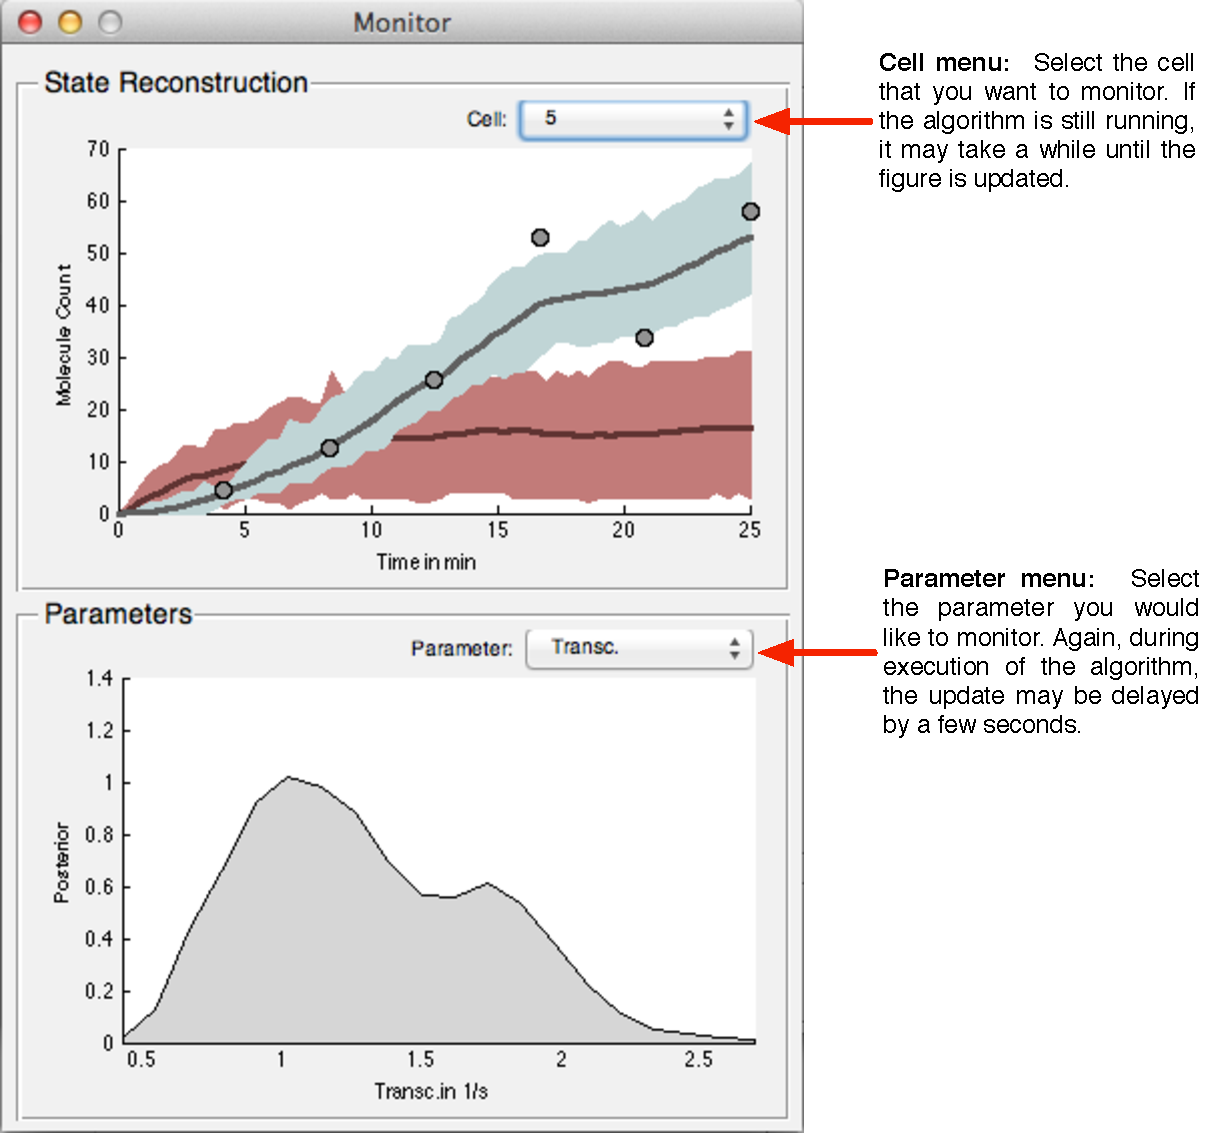
\includegraphics[width=0.5\textwidth]{figures/Doc_Monitor}
\caption{Monitoring the simulations.}
\label{fig:Monitor}
\end{center}
\end{figure}


\paragraph{Export:} After the algorithm has finished, you can export the inferred parameter statistics. Press the \textit{Export} button to specify and save the destination file. The exported file can be easily loaded into MATLAB for further analysis. More specifically, it will contain a structure \textit{Stat}, containing the prior and posterior statistics for all parameters (i.e., the mean values and the $0.05$ and $0.95$ quantiles).

\paragraph{Example Data:} The toolbox comes with two exemplary datasets: 
\begin{enumerate}
	\item \textbf{Synthetic data:} A synthetic dataset generated using the \textit{Simple Expression Model} and a double-pulse input stimulus. The corresponding files can be found in the folder \textit{PATH/ExampleData/SimpleModel/}. Additionally, you can find the associated MATLAB scripts that were used to generate the data.
	\item \textbf{GAL1 data:} An experimental dataset from the study in \cite{Zechner2013}. It consists of measurements of a fluorescent reporter that is expressed upon translocation of the transcription factor \textit{GEV}. The \textit{GEV} translocation was also experimentally measured and acts as the temporal input to the stochastic model. The corresponding files can be found in the folder \textit{PATH/ExampleData/GAL1/}.
\end{enumerate}

\paragraph{Step-by-step Example:}
\begin{enumerate}
	\item Execute the file \textit{PATH/GUI/StartGUI.m}. The main window will pop up.
	\item Per default, the kinetic model drop-down menu will be set to \textit{Simple Expression Model} and the parameter table will show the corresponding parameters. Keep all parameter values as initialized.
	\item In the panel \textit{Transcriptional Activation (Input)} select \textit{Temporal} and load the file \\ \textit{PATH/ExampleData/SimpleModel/InputSimpleModel.mat}. The input profile will be displayed in the corresponding figure.
	\item In the panel \textit{Protein Measurements (Output)} select and load the file \\ \textit{PATH/ExampleData/SimpleModel/MeasurementsSimpleModel.mat}. The measurements will be displayed in the corresponding figure.
	\item For a quick illustration, set the number of particles to $200$. This will result in a short simulation time but keep in mind that the resulting posterior distributions are likely to be degenerate (see section \ref{sec:Degeneracy}). Keep all other parameters as initialized. 
	\item Press \textit{Run!}. The algorithm will start and the monitor window pops up. You can use the corresponding drop-down menus to choose between different cells and parameters. 
	\item In case you want to abort the simulations, press \textit{Stop!}.
	\item Once the algorithm has finished, press \textit{Export} to save your results.
\end{enumerate}

\section{The \DPP Toolbox}

\DPP is a MATLAB toolbox for the inference of stochastic chemical reaction networks using time-lapse single-cell data. In contrast to \GuiDPP, it is fully general and applies to arbitrary biochemical systems.

\subsection{How to Use \DPP}
\label{sec:DPP}
In the following, we explain the functionality of \DPP using an exemplary MATLAB script. A similar script is delivered with the toolbox, which is located in the root directory (i.e., \textit{PATH/InferenceDPP.m}). The goal of the script is to infer stochastic gene expression dynamics from heterogeneous single-cell data using \DPP. 

\paragraph{Setting path dependencies:}

\DPP requires certain library paths to be set. In particular, it will use functions located in the folder \textit{PATH/Common/*} and the model specifications in \textit{PATH/Models/}. Any additional libraries can be added analogously. Figure \ref{fig:Paths} shows the corresponding code lines.

\begin{figure}[ht!]
\begin{center}
	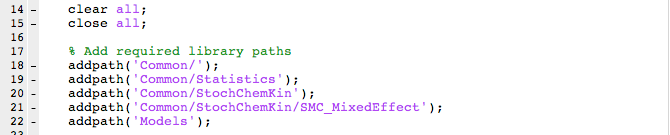
\includegraphics[width=0.6\textwidth]{figures/Doc_Paths}
\caption{Setting the path dependencies.}
\label{fig:Paths}
\end{center}
\end{figure}

\paragraph{Initialize model and input:}

The script is based on the \textit{Two-State Model} described in Section \ref{sec:HowToGuiDPP}. In line 27 of Figure \ref{fig:Model}, the model specification is imported. Subsequently, a structure \textit{kineticModel} will be available in MATLAB's \textit{Workspace}. Since the example code is based on synthetic data, a temporal input profile needs to be synthesized. In this case, we simulate a double-pulsed induction of the target gene. The input profile is represented by a piece-wise constant function. The corresponding structure \textit{inputParams} is characterized by three fields:
	\begin{itemize}
		\item \textit{inputTimes:} Specifies the time points where the input profile changes. The initial time point (i.e., $t=0$) is not included.
		\item \textit{inputLevels:} Specifies the magnitude of the input profile. At time $t=0$, the magnitude of the input profile is set to the first value in \textit{inputLevels}. At the time point corresponding to the first entry in \textit{inputTimes}, the input profile changes to the second value in \textit{inputLevels} and so on. Make sure that the timespan of your input profile is at least as large as the duration of the experiment.
		\item \textit{inputRateIndex:} Defines the index of the reaction that is modulated by the input profile. In particular, the effective propensity will computed as $h(x, t)=c_{i} u(t) g_{i}(x)$, with $i=inputRateIndex$.
	\end{itemize}
	
Lines 36-39 show the corresponding code from the example script. Note that \textit{inputRateIndex} is part of the model specification and hence, the corresponding field in the \textit{inputParams} structure is set to this value.

\begin{figure}[htbp]
\begin{center}
	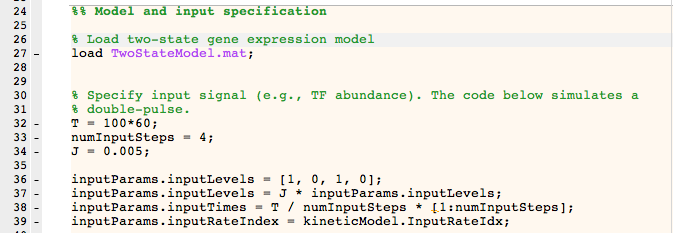
\includegraphics[width=0.6\textwidth]{figures/Doc_Model}
\caption{Model and input initialization.}
\label{fig:Model}
\end{center}
\end{figure}

\paragraph{Constructing a general state-space model:}

\DPP combines the kinetic model specification with further properties of the experiment to construct a general mixed-effect state-space model. These properties include specifications of the population heterogeneity, prior distributions or the measurement noise model. The corresponding code can be found in Figure \ref{fig:Statespace}. In line 44, the output-weight matrix is constructed. This defines the set of species (or linear combinations thereof) that were measured during the experiment. Hence, the measured quantities at a certain time point are given by $W^{T} X_{l}$. 
Since the given code example is based on synthetic data, the measurement time points need to be defined (lines 52-53). In contrast, if experimental data is used, those have to be set to the underlying acquisition time points. \newline

In some cases it might be desired to assume certain kinetic parameters to be known a priori. Hence, the rate constants that are to be estimated from the data need to be specified (line 58). All other rate constants will be set to the values of model specification (i.e., the structure \textit{kineticModel}).

For the remaining parameters, prior distributions need to be specified. The current implementation supports Gamma-type prior distributions $\GammaDistribution(a, b)$. Lines 67-68 specify the prior distributions corresponding to the previously defined reactions. Accordingly, the heterogenous reaction (in this case the translation rate) is selected to be heterogeneous. Note that in the current release, only one reaction can be heterogenous. If you wish the model to be entirely homogenous, set all values in \textit{randomEffect} to zero. Note that for the heterogeneous reaction, the corresponding values $a$ and $b$ of the prior distribution are ignored during the inference. However, when using synthetic data, they are used for simulating the heterogeneity. Hence, the values $a$ and $b$ correspond to the ground-truth and accordingly, each cell's heterogeneous parameter will be randomly drawn from $\GammaDistribution(a, b)$. If a heterogenous reaction was selected, the bivariate log-normal hyperprior distribution over $(a, b)$ needs to be specified. The two parameters \textit{MuHyper} and \textit{SigmaHyper} are defined in lines 76-78. \newline

If morphological features are used for the inference, the morphological parameters $\rho$ and $\phi$ need to be specified. The morphological parameters are assumed to be noisy readouts of the extrinsic factors specified by the distribution $\GammaDistribution(\rho, \phi z)$, with $z$ as the extrinsic factor. Note that in this case, the morphological readout scales inversely with $z$, and hence, if the morphological feature is hypothesized to be positively correlated with the extrinsic factor, it should be inverted beforehand (i.e., such as might be the case for the cell-size). In case no morphological features are used, set \textit{MorphParams = [];}, \textit{MuMorph = [];} and \textit{SigmaMorph = [];}. If you would like to use the morphological features but you already know $\rho$ and $\phi$ (maybe from a previous experiment), set \textit{MorphParams} to the desired values and \textit{MuMorph = [];} and \textit{SigmaMorph = [];}. In order to estimate the morphological parameters from the measurements, \textit{MuMorph} and \textit{SigmaMorph} define the log-normal hyperprior distribution over $\rho$ and $\phi$ (see lines 87-89). During inference, the values specified in \textit{MorphParams} will be ignored but will be used to simulate the morphological readouts in case of synthetic data. \newline

Lines 95-96 define the measurement noise model. \DPP supports either normal or log-normal measurement densities. In case of normal distribution (\textit{mDens = 'normal';}), the measurements are assumed to stem from a Gaussian distribution centered around the true value with a certain standard deviation, i.e., $Y_{l} \sim N(W^{T} X_{l}, \sigma)$. For a log-normal error model (\textit{mDens = 'logn';}), the measurements are assumed to be given by $Y_{l} \sim N(W^{T} X_{l}, s)$, with $s$ as a scaling parameter. The vector \textit{measurementParams} must contain either one or three values, depending on if the scaling parameter (either $\sigma$ or $s$) of the noise shall be estimated from the data. If the scaling parameter is known, set \textit{measurementParams} to the respective value. The scaling parameter is estimated, if \textit{measurementParams} is a 1-by-3 vector, where the latter two entries specify the inverse-Gamma prior distribution (such as described in Section \ref{sec:HowToGuiDPP}). Again, the first entry will then be ignored during inference, but will be used for generating the synthetic data (i.e., specifies the ground-thruth value). \newline

Given the previous definitions, the state-space model structure can be instantiated by calling the function \textit{InitializeMEGSM} (see lines 98-101).

\begin{figure}[htbp]
\begin{center}
	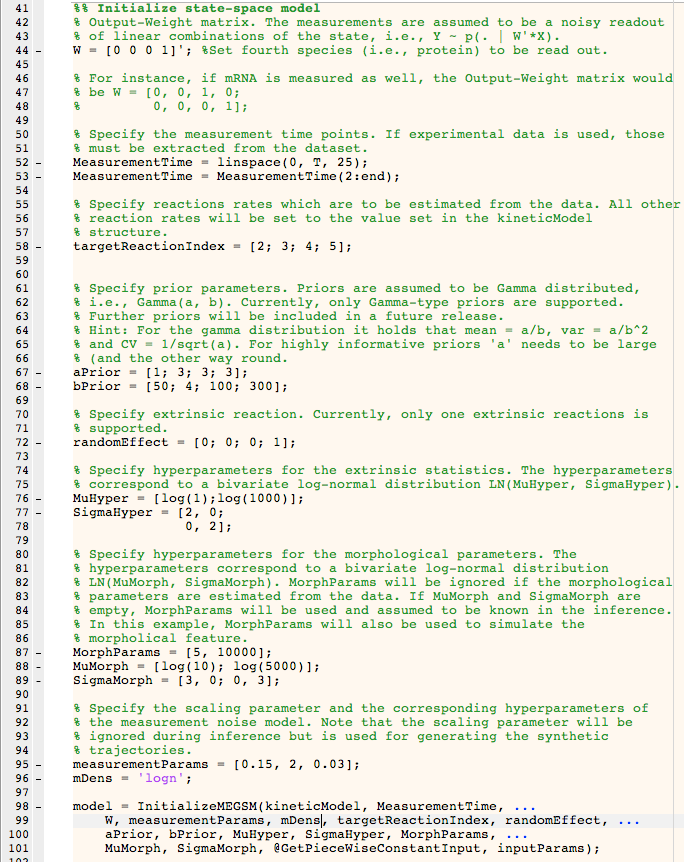
\includegraphics[width=0.6\textwidth]{figures/Doc_Statespace}
\caption{Constructing a general state-space model.}
\label{fig:Statespace}
\end{center}
\end{figure}

\paragraph{Load / simulate experimental data:}

If synthetic data shall be used for the inference, you can call the \textit{SimulateCells} function (see lines 101-102 in Figure \ref{fig:TargetData}). The resulting trajectories and morphological features are simulated according to the defined state-space model and returned in the cell-array \textit{cells}. Each entry of that array corresponds to one cell and includes the corresponding measurement trajectory, the morphological readout as well as the exact realization of the underlying Markov chain. In case you want to use experimental data, you need to construct the cell-array accordingly. In particular, a valid cell-structure contains the fields:
\begin{enumerate}
	\item \textit{MeasurementTime:} The vector containing the measurement time points.
	\item \textit{Measurement:} The measured protein abundance at the measurement time points defined above.
	\item \textit{Simulated:} Zero if the data was measured experimentally and one if it was simulated.
	\item \textit{MorphologicalFeatureValue:} If morphological features are used, this field stores the value of the morphological feature.
	\item \textit{xPath:} Synthetic data only. Stores the exact species abundance of the underlying Markov chain.
	\item \textit{tPath:} Synthetic data only. Contains the jump times of the underlying Markov chain.
	\item \textit{rPath:} Synthetic data only. Contains the reaction indices that happened at the jump times.
\end{enumerate}
In the folder \textit{PATH/ExampleData/} you find exemplary \textit{.mat} files containing valid cell structures.

Once loaded, the cells can be visualized using the function \textit{PlotCells} (see Figure \ref{fig:TargetData})

\begin{figure}[htbp]
\begin{center}
	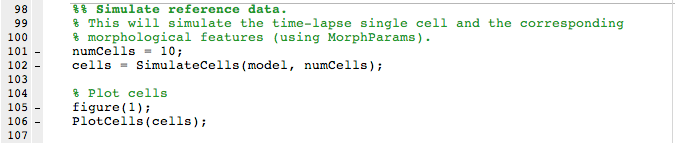
\includegraphics[width=0.6\textwidth]{figures/Doc_TargetData}
\caption{Load / simulate experimental data.}
\label{fig:TargetData}
\end{center}
\end{figure}

\paragraph{Set options for inference and plotting:}

\DPP requires several properties to be specified before it can be run.There are three different structures associated with different properties of the algorithm. \newline

The algorithm configuration is defined in the structure \textit{options} (lines 125-143). A default options structure can be created using the function \textit{CreateDPPOptions}. The structure consists of the following fields:
\begin{enumerate}
	\item \textit{M:} The number of particles used for inference.
	\item \textit{BurnIn:} The burn-in period of the MCMC sampler. During each time-iteration, the first $K$ samples will be discarded, where $K$ corresponds to the value of \textit{BurnIn}.
	\item \textit{StorePathCellIdx:} Specifies the indices of the cells whose state trajectories shall be stored. Note that the required memory increases with the number of cells specified in \textit{StorePathCellIdx}.
	\item \textit{BlockSize:} In order to save memory, the algorithm implements a block-processing mode, where one block of size \textit{BlockSize} is processed at once.
	\item \textit{Plot:} \textit{Plot=0} won't produce any monitoring plots. If \textit{Plot=1}, figures with the most recent parameter and state distributions will be shown after each time-iteration. 
	\item \textit{NumMeasurements:} By setting this variable, the algorithm will only consider the first \textit{NumMeasurements} measurement time points. If the variable is not specified, all time points will be used.
	\item \textit{StorePathNumPoints:} Set to zero in order to store the full sample paths of the Markov chain. Set to a value greater than zero to down-sample the paths to the desired number of values.
\end{enumerate}

The parameters for plotting the reconstructed state distributions are specified in the structure \textit{qPlotOptions} (lines 119-123). A default options structure can be created using the function \textit{CreatePlotOptions}. You can pass an array of Figures-handles to the function in order to plot the reconstruction into custom windows Otherwise, a figure is created automatically during runtime. The structure consists of the following fields:
\begin{enumerate}
	\item \textit{quantile:} A vector containing two quantiles that are plotted as credible intervals. The default value is $[0.05, 0.95]$.
	\item \textit{plotReferenceCells:} Set to one if you wish to display the measured cells and to zero otherwise.
	\item \textit{stateIdx:} Specify a vector of indices of chemical species you want to visualize.
	\item \textit{cellIdx:} Provide the indices of the cells you want to visualize. Note that those each of those indices must also be provided in the \textit{options.StorePathCellIdx} vector.
	\item \textit{FigureHandlesCells:} A set of figure handles, each of them corresponding to one of the cells in \textit{cellIdx}. The reconstructed states will be plotted using the given handles.
	\item \textit{plotConfidence:} Specify whether you wish to visualize the credible intervals given in \textit{quantile}.
	\item \textit{numPoints:} The number of sampling points along the full measurement time interval. Note that for large \textit{numPoints}, plotting of the reconstructed paths may take a while.
\end{enumerate}

\begin{figure}[htbp]
\begin{center}
	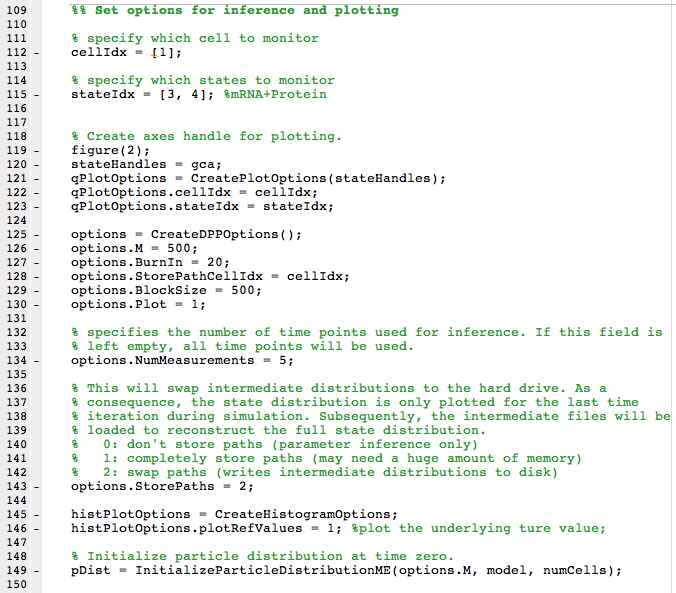
\includegraphics[width=0.6\textwidth]{figures/Doc_Options}
\caption{Constructing a general state-space model.}
\label{fig:Options}
\end{center}
\end{figure}

\paragraph{Run inference:}

The main inference algorithm can be started using the function \textit{RunDPP} (see Figure \ref{fig:Inference}). The function is called using the previously defined model and options and returns the inferred posterior distribution in \textit{pDist} (line 161). Note that the execution time of the algorithm strongly depends on the number of particles and cells. Subsequently, if the intermediate data were swapped to the hard-drive, the full posterior distribution over the paths is reconstructed and plotted (lines 166-171). You can then use the posterior distribution for further analysis. For instance you can use the function \textit{GetParameterStatistics} to compute the prior and posterior statistics for the inferred parameters. The results are return in the structure \textit{ParametersStats} (line 174). 

\begin{figure}[htbp]
\begin{center}
	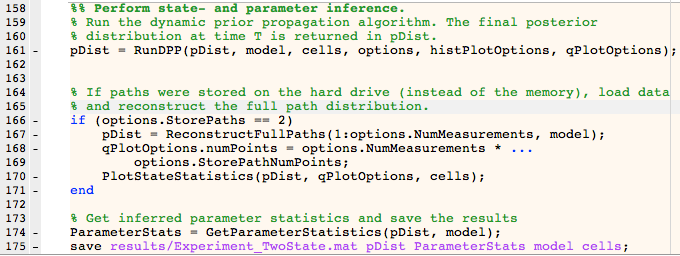
\includegraphics[width=0.6\textwidth]{figures/Doc_Inference}
\caption{Run inference.}
\label{fig:Inference}
\end{center}
\end{figure}


\section{Practical Hints}

\subsection{Generating new models}
\label{sec:Models}

You can easily add your own kinetic models to \DPP and \GuiDPP using a simple MATLAB script. Models are defined by a MATLAB structure \textit{kineticModel} with the following fields
\begin{enumerate}
	\item \textit{Name:} A string specifying the name of the model. This name will be shown in the corresponding drop-down menu in \GuiDPP.
	\item \textit{Pre:} A $m\times n$ matrix defining the left-hand-side of your reaction system (i.e., the reactants). $m$ corresponds to the number of reactions and $n$ to the number of chemical species.
	\item \textit{Post:}  A $m\times n$ matrix defining the right-hand-side of your reaction system (i.e., the products). $m$ corresponds to the number of reactions and $n$ to the number of chemical species.
	\item \textit{S:} The stoichometry matrix defined by $Post-Pre$.
	\item \textit{c:} An $m \times 1$ vector containing nominal rate constants for each reaction.
	\item \textit{X0:} An $n\times 1$ vector containing the initial conditions of the reaction system.
	\item \textit{NumSpecies:} The number of species $n$.
	\item \textit{NumReactions:} The number of reactions $m$.
	\item \textit{SpeciesNames:} A $n\times1$ list of strings containing the species names. Note that if used with \GuiDPP, the species \textit{mRNA} and \textit{Protein} need to be part of the model.
	\item \textit{ReactionNames:} A $m\times1$ list of reaction names.
	\item \textit{InputRateIdx:} The index of the reaction that is modulated by an external stimulus. This field is required even if no (i.e., a constant) input is used.
\end{enumerate}
Once the model has been created in MATLAB, save it to the \textit{PATH/Models/} folder using the MATLAB command \textit{save}. Please consult the example scripts \textit{CreateSimpleModel.m} and \textit{CreateTwoStateModel.m} in the folder \textit{PATH/Models/} for further information.

\subsection{Static time-delays between induction and expression} In many applications involving fluorescent reporter proteins, a static time-delay between induction and expression is observed. While such delays can in principle be achieved by including multiple sequential first-order events in the kinetic model, the resulting inference problems becomes challenging due to the increased parameter- and state-space. A simple and pragmatic approach is to detect the time-point at which the increase of the protein abundance is statistically significant and to discard the measurements before that time-point. For instance, a one-sided Kolmogorov-Smirnoff test can be performed to detect that time-point at a given significance level \cite{Zechner2013}.

\subsection{Sample degeneracy} \label{sec:Degeneracy} \DPP and \GuiDPP rely on a sequential Monte-Carlo inference scheme, which - like all sampling-based methods - produce reasonable results only if \textit{enough} samples (i.e., particles) are used. It is generally hard to provide guidelines on how to choose an appropriate number of particles since that number strongly depends on several factors such as the system dynamics, the prior knowledge or the measurement noise model -- to name a few. However, there are certain indicators that may tell you if the number of particles is too small. For instance, sequential Monte-Carlo procedures will in such case yield \textit{degenerate} solutions, i.e., the final distribution consists of only very few different particles. An exemplary degenerate posterior distribution is shown in Figure \ref{fig:Degeneracy}. It can be seen that the for the early time points, the posterior distribution consists of only a single sample path, because all other particles were lost during the subsequent time iterations. Be aware that very narrow posterior distributions do not necessarily mean accurate inference results. In many cases they rather indicate sample degeneracy such that the number of particles must be increased.


\begin{figure}[htbp]
\begin{center}
	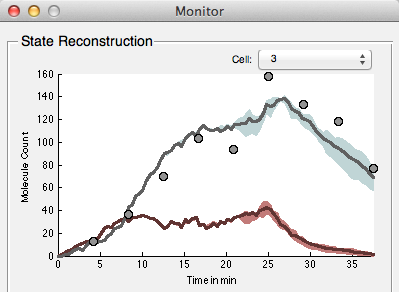
\includegraphics[width=0.4\textwidth]{figures/Doc_Degenaracy}
\caption{Example of a degenerate posterior distribution.}
\label{fig:Degeneracy}
\end{center}
\end{figure}

\subsection{Choosing your priors} \label{sec:Priors} In order to run \DPP you have to provide prior distributions over the unknown parameters. According to the Bayesian philosophy, such priors should not be considered as tuning variables, but should rather reflect what is known about the parameters a priori. Nevertheless, the algorithm performance strongly depends on such prior knowledge which should therefore be incorporated wherever possible. For instance, rate constants are generally constrained by biophysical laws. While exact limits are typically unknown, it is often straight-forward to roughly define plausible ranges. As discussed above, \DPP assumes Gamma-type prior distributions over the kinetic parameters. On the one hand, the Gamma distribution turns out to be very useful for biological applications since it represents a very versatile distribution for the positive orthant -  ranging from highly over-dispersed and right-tailed to under-dispersed and symmetric distributions. On the other hand, the Gamma distribution has convenient mathematical properties which allow to run \DPP without approximations.

The Gamma distribution is fully specified by a shape parameter $a$ and a scaling parameter $b$. Since those values are generally hard to interpret, it is more convenient to transform them into a set of standard statistics. For instance, mean and variance of a Gamma distribution are given by $m = \frac{a}{b}$ an $s = \frac{a}{b^{2}}$ respectively. Furthermore, the coefficient of variation (CV) is given by $CV=\frac{1}{\sqrt{a}}$. Hence, if a parameter is well-known a-priori, the variance (and CV) will take very small values. In contrast, if only few information is available, the variance and CV will be large. Hence, for a given mean and variance (or CV) you can specify $a$ and $b$ by 
\begin{equation}
	a = \frac{m^2}{s} \quad\quad b =\frac{m}{s}
\end{equation}
or 
\begin{equation}
	a = \frac{1}{CV^2} \quad \quad  b = \frac{1}{CV^2 m}.
\end{equation}

{\footnotesize
\begin{thebibliography}{1}

\bibitem{Zechner2013}
C Zechner, M Unger, S Pelet, M Peter, and H
  Koeppl (2014).
\newblock Scalable inference of heterogeneous reaction kinetics from pooled single-cell recordings.
\newblock Nature Methods.
\newblock In press.

\end{thebibliography}}


\end{document}  
